\documentclass{article}

\usepackage{minted}
\usepackage{xcolor} % to access the named colour LightGray
\definecolor{LightGray}{gray}{0.9}

% Language setting
% Replace `english' with e.g. `spanish' to change the document language
\usepackage[english]{babel}

\usepackage{amsfonts}
\usepackage{tikz}
%\usetikzlibrary{shapes,arrows,positioning}
\usetikzlibrary{automata,arrows,positioning,calc}

\usepackage{listings}

% Set page size and margins
% Replace `letterpaper' with `a4paper' for UK/EU standard size
\usepackage[letterpaper,top=2cm,bottom=2cm,left=3cm,right=3cm,marginparwidth=1.75cm]{geometry}

% Useful packages
\usepackage{amsmath}
\usepackage{graphicx}
\usepackage[colorlinks=true, allcolors=blue]{hyperref}
\setcounter{secnumdepth}{0}
\title{Optiver questions}

\begin{document}

\noindent Blah blah blah, some very engaging blurb.

\section{Problem outline}
An ant leaves its anthill in order to forage for food. It moves with the speed of 10cm per second, but it doesn't know where to go, therefore every second it moves randomly 10cm directly north, south, east or west with equal probability.

\subsection{Question 1}
If the food is located on east-west lines 20cm to the north and 20cm to the south, as well as on north-south lines 20cm to the east and 20cm to the west from the anthill, how long will it take the ant to reach it on average?

\subsection{Answer}
On average, it will take ant \textbf{4.5} seconds to reach the food boundary.

\subsection{Analytical solution}
There are many ways to approach this problem. I decided to use results from the Markov Chains theory. I started by drawing out all the states with their probabilities. I defined the boundary as the absorbing state 0. State number 5 represents the starting point of the ant. 

\begin{center}
	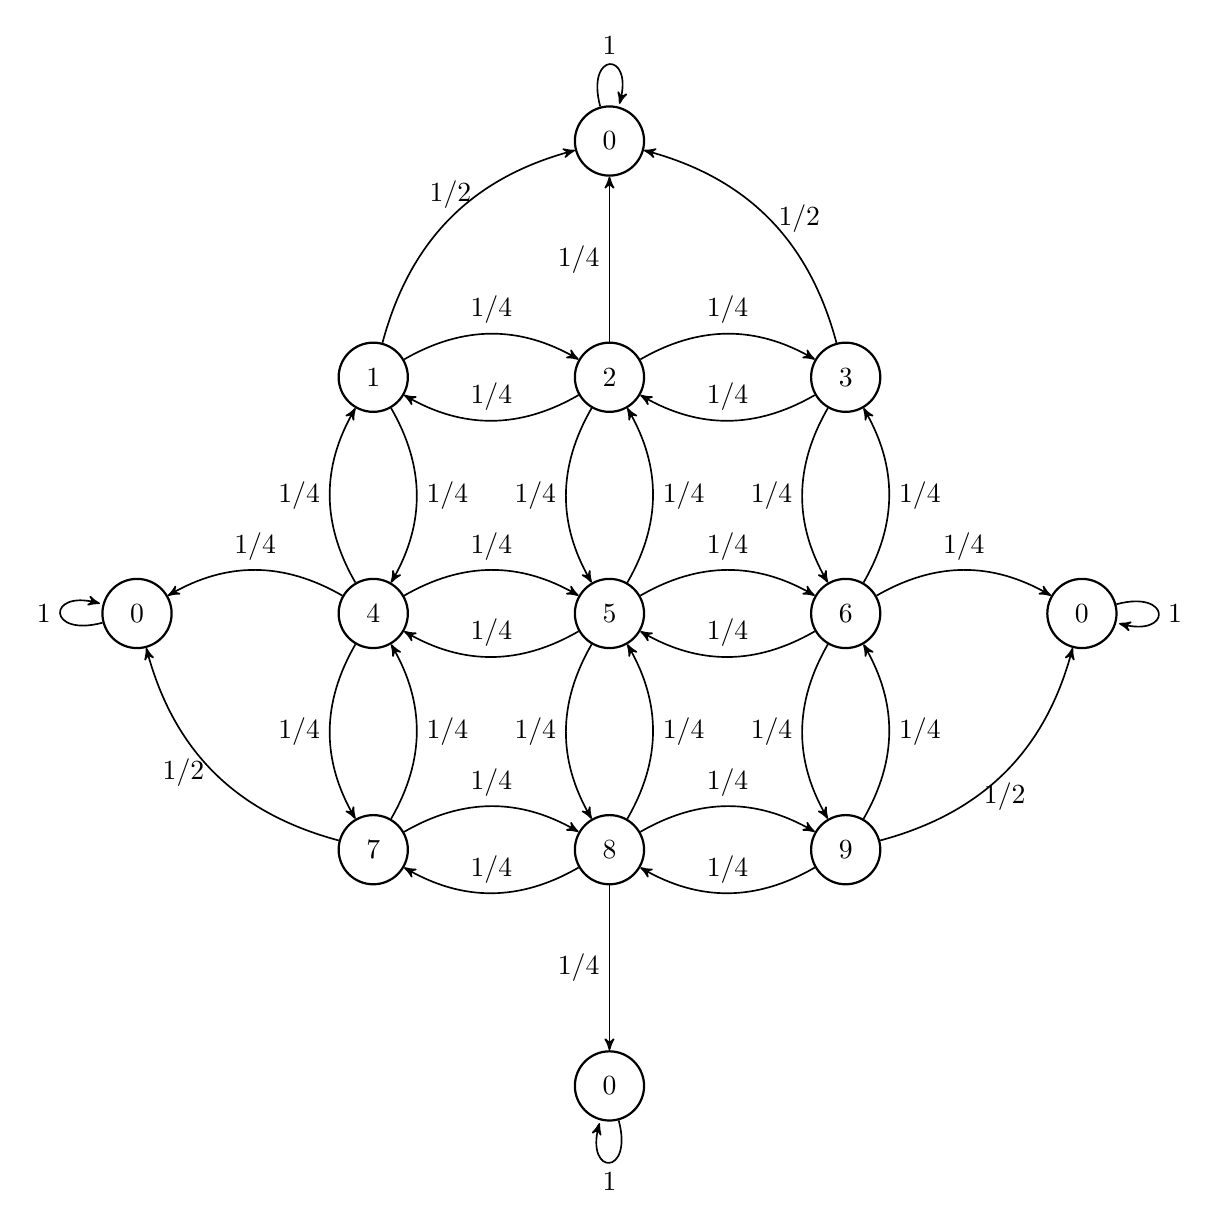
\begin{tikzpicture}[->, >=stealth', auto, semithick, node distance=3cm]
	\tikzstyle{every state}=[fill=white,draw=black,thick,text=black,scale=1]
	\node[state]    (A)               {$0$};
	\node[state]    (B)[left of=A, below of=A]   {$1$};
	\node[state]    (C)[right of=B]   {$2$};
	\node[state]    (D)[right of=C]   {$3$};
	
	\node[state]    (E)[below of=B]   {$4$};
	\node[state]    (F)[below of=C]   {$5$};
	\node[state]    (G)[below of=D]   {$6$};
	
	\node[state]    (H)[below of=E]   {$7$};
	\node[state]    (I)[below of=F]   {$8$};
	\node[state]    (J)[below of=G]   {$9$};
	
	\node[state]    (K)[left of=E]     {$0$};
	\node[state]    (L)[right of=G]     {$0$};
	\node[state]    (M)[below of=I]     {$0$};
	
	\path
	(A) edge[loop above, above]			node{$1$}	(A)
	(B) edge[bend left,above]	node{$1/2$}	(A)
	edge[bend left, above]		node{$1/4$}	(C)
	edge[bend left, right]     node{$1/4$} (E);
	
	\path
	(C) edge[left]			node{$1/4$}	(A)
	(C) edge[bend left,above]	node{$1/4$}	(B)
	(C) edge[bend left,above]	node{$1/4$}	(D)
	(C) edge[bend right, left]	node{$1/4$}	(F);
	
	\path
	(D) edge[bend right, right]			node{$1/2$}	(A)
	(D) edge[bend left,above]	node{$1/4$}	(C)
	(D) edge[bend right, left]	node{$1/4$}	(G);
	
	
	\path
	(K) edge[loop left, left] node{$1$} (K)
	(E) edge[bend left,left]	node{$1/4$}	(B)
	(E) edge[bend right, above]			node{$1/4$}	(K)
	(E) edge[bend left,above]	node{$1/4$}	(F)
	(E) edge[bend right, left]	node{$1/4$}	(H);
	
	\path
	(F) edge[bend right,right]	node{$1/4$}	(C)
	(F) edge[bend left, above]			node{$1/4$}	(E)
	(F) edge[bend left,above]	node{$1/4$}	(G)
	(F) edge[bend right, left]	node{$1/4$}	(I);
	
	\path
	(L) edge[loop right, right] node{$1$} (L)
	(G) edge[bend left,above]	node{$1/4$}	(F)
	(G) edge[bend right, left]			node{$1/4$}	(J)
	(G) edge[bend right, right]			node{$1/4$}	(D)
	(G) edge[bend left, above]			node{$1/4$}	(L);
	
	\path
	(H) edge[bend right,right]	node{$1/4$}	(E)
	(H) edge[bend left, above]			node{$1/4$}	(I)
	(H) edge[bend left, left]			node{$1/2$}	(K);
	
	\path
	(M) edge[loop below, below]  node{$1$} (M)
	(I) edge[bend left,above]	node{$1/4$}	(H)
	(I) edge[bend left, above]			node{$1/4$}	(J)
	(I) edge[bend right, right]			node{$1/4$}	(F)
	(I) edge[left]			node{$1/4$}	(M);
	
	\path
	(J) edge[bend right,right]	node{$1/4$}	(G)
	(J) edge[bend left, above]			node{$1/4$}	(I)
	(J) edge[bend right, below]			node{$1/2$} (L)
	;
	
	%\node[above=0.5cm] (A){Patch G};
	%\draw[red] ($(D)+(-1.5,0)$) ellipse (2cm and 3.5cm)node[yshift=3cm]{Patch H};
	\end{tikzpicture}
\end{center}

This Markov Chain has exactly one absorbing state, therefore, we can use the well known result to compute the expected absorption time for each state. $$\mu_i=1 + \sum_j p_{ij}\mu_j$$

Probability of transitioning from state $i$ to state $j$ is denoted as $p_{i,j}$, and expected absorption time of state $i$ is denoted as $\mu_i$. 

Applying this formula to the diagram above yields the following system of linear equations, which can be solved using classical linear algebra techniques.
\begin{align}
    1 &= \mu_0\\
    1 &= \mu_1  - 1/4(\mu_2 + \mu_4)\\
    1 &= \mu_2 - 1/4(\mu_1 + \mu_3 + \mu_5)\\
    1 &= \mu_3 - 1/4(\mu_2 +\mu_6) \\
    1 &= \mu_4 - 1/4(\mu_1+\mu_5+\mu_7)\\
    1 &= \mu_5 - 1/4(\mu_2+\mu_4+\mu_6 +\mu_8)\\
    1 &= \mu_6 - 1/4(\mu_3 +\mu_5+\mu_{9}) \\
    1 &= \mu_7 - 1/4(\mu_4 + \mu_8) \\
    1 &= \mu_8 - 1/4(\mu_5 + \mu_7 + \mu_{9})\\
    1 &= \mu_{9} - 1/4(\mu_6 + \mu_8)
\end{align}

After solving the $Ax=b$ problem, I obtained $\mu_5=4.5$, which implies that on average it will take 4.5 seconds to reach the food boundary. 


Solution of the system of linear equations:
$\mu_0 = 1, \mu_1 = 2.75, \mu_2 = 3.5, \mu_3= 2.75, \mu_4 = 3.5, \mu_5 = 4.5, \mu_6 = 3.5, \mu_7 = 2.75, \mu_8 =3.5, \mu_9 = 2.75$


\subsection{Question 2}
What is the average time the ant will reach food if it is located only on a diagonal line passing through (10cm, 0cm) and (0cm, 10cm) points?

\subsection{Answer}
Since there is a positive probability to always move left, this implies that expected time to reach the line of food is \textbf{infinite}.

\subsection{Analytical proof}
We start by observing that the expected number of steps is non-negative, as it is a simple non-decreasing counter. We use this fact to restrict this problem to one dimension, and show that on an integer grid, expected time for the random walk to reach any point $(x,y)$ from the origin $(0,0)$ is infinite. This can be shown by contradiction. 
\\~\\
\noindent Let $T$ be the expected number of steps to travel from 0 to 1 (the 1-dimensional setting). If you go +1 (right), you are done, however if you -1 (left) you will have to make $2T$ steps to reach 1. So, half of the time you will be done in one step, the other half of the time you make one step and then have to travel $2T$ to reach the end point. Therefore, $T=\frac{1}{2}(1) + \frac{1}{2}(1+2T) = 1 + T$, which is a contradiction for finite $T$.


\subsection{Question 3}
Can you write a program that comes up with an estimate of average time to find food for any closed boundary around the anthill? What would be the answer if food is located outside an defined by $( (x – 2.5\text{cm}) / 30\text{cm} )^2 + ( (y – 2.5\text{cm}) / 40\text{cm} )^2 < 1$ in coordinate system where the anthill is located at $(x = 0\text{cm}, y = 0\text{cm})$? Provide us with a solution rounded to the nearest integer.

\subsection{Answer}
The ant takes \textbf{14} seconds (rounded to the nearest integer) to reach the food boundary

\subsection{Implementation}
I used Python to implement a simple random walk simulator. There are two files $main.py$ and $boundary.py$. The latter file is used to define an arbitrary 2D boundary, using a function that returns True if a given point has left the region and False otherwise. This was done to make my simulation code boundary-agnostic, and allow for an easy definition of an 2D arbitrary boundary. The $main.py$ file is a parallelised solver. The key function is $do\_process$ which repeats the simulation $n$ times and then returns the total sum of the number of steps taken to reach the boundary. The final average is computed as $$\frac{\Sigma_{process}(\text{total sum from the process})}{(\text{number of processes})\times(\text{number of iteration per process})}$$
\\~\\
main.py : https://github.com/daily-etymology/optiver-application/blob/main/main.py\\
boundary.py : https://github.com/daily-etymology/optiver-application/blob/main/boundary.py

\end{document}
